\documentclass[12pt]{article}

%\usepackage{graphicx}
\usepackage[dvipsone]{graphicx}
\usepackage{subfigure}
\usepackage{pslatex}
\usepackage{listings}
%\usepackage{multind}
%\usepackage{showidx}
\usepackage{graphics}
\usepackage{epsf}
\usepackage{epsfig}
\usepackage{multirow}
\usepackage{amsmath}
\usepackage[hyphens,obeyspaces,spaces]{url}
%\usepackage{hyperref}
%\usepackage{breakurl}
\usepackage{alltt}
%\usepackage[pdftex]{hyperref}
%\usepackage{xfrac}


%%% Formatting options
%\usepackage[colorlinks=true]{hyperref}
%\setlength{\parindent}{0em}
%\setlength{\parskip}{1em}

%%% Title/author options
\title{Deploying IP-based Emergency Services}
\author{
Internet Architecture Board 
}
\date{}


\begin{document}

\maketitle

\begin{abstract}
The IETF ECRIT and GEOPRIV working groups have developed standards
for critical components of the next-generation, IP-based 911 system.
This whitepaper reviews some of the basic principles of these technologies
and explains how to incrementally deploy the architecture to take into account currently deployed emergency services systems.  
\end{abstract}


\pagebreak



\section{Introduction}
\index{SIP|(}
\index{LoST|(}
\index{Organizations and Groups!IETF|(}
\index{Organizations and Groups!Geopriv|(}
\index{Organizations and Groups!ECRIT|(}
The ability to summon the police, the fire department or an ambulance in emergencies is one of the most important functions available when using the telephone. As telephone functionality moves from circuit-switched to Internet telephony, its users rightfully expect that this core feature will continue to be available and work as well as it has in the past.  Users also expect to be able to reach emergency assistance using new communication devices and applications, such as instant messaging or \index{SMS}\index{SMS}SMS, and new media, such as video. In all cases, the basic objective is the same: The person seeking help needs to be connected with the most appropriate public safety answering point (PSAP), where call takers dispatch assistance to the caller's location. PSAPs are responsible for a particular geographic region, which can be as small as a single university campus or as large as a country. 

The transition to Internet-based emergency services introduces two major structural challenges. First, while traditional emergency calling imposed no requirements on end systems and was regulated at the national level, Internet-based emergency calling needs global standards, particularly for end systems. In the old public switched telephone network (\index{PSTN}PSTN), each caller used a single entity, the landline or mobile carrier, to obtain services. For Internet multimedia services, network level transport and application can be separated, with the Internet service provider (ISP)  providing IP connectivity service, and a voice service provider (VSP)  adding call routing and \index{PSTN}PSTN termination services. We ignore the potential separation between the Internet access provider, i.e., a carrier that provides physical and data link layer network connectivity to its customers, and the ISP that provides network layer services. We use the term VSP for simplicity, instead of the more generic term Application Server Provider (ASP). 

The documents that are being developed within the IETF Emergency Context Resolution with Internet Technology (ECRIT) working group~\cite{ecrit-wg} support multimedia-based emergency services, and not just voice. As will be explained in more detail below, emergency calls need to be identified for special call routing and handling services, and they need to carry the location of the caller for routing and dispatch. Only the calling device can reliably recognize emergency calls, while the ISP is a reliable source of location information of the calling device based on its point of attachment to the network. Handling of emergency calls is, however, complicated by the wide variety of access technologies in use, such as virtual private networks (\index{VPN}\index{VPN}VPNs), other forms of tunneling, firewalls, and Network Address Translators (\index{NAT}\index{NAT}NATs).

The emergency services architecture developed by the IETF ECRIT working group is described in~\cite{rfc6443} and can be summarized as emergency calls are generally handled like regular multimedia calls, except for call routing. The ECRIT architecture assumes that PSAPs are connected to an IP network and support the Session Initiation Protocol (\index{SIP}SIP)~\cite{rfc3261} for call setup and messaging. However, the calling user agent may use any call signaling or instant messaging protocol, which the VSP then translates into \index{SIP}SIP.

Non-emergency calls are routed by a VSP, either to another subscriber of the VSP, typically via some \index{SIP}SIP session border controller or proxy, or a \index{PSTN}PSTN gateway. For emergency calls, the VSP keeps its call routing role, routing calls to the emergency service system, to reach a PSAP, instead. However, we also want to allow callers that do not subscribe to a VSP to reach a PSAP, using nothing but a standard \index{SIP}SIP~\cite{rfc3261} user agent (see~\cite{draft-ietf-ecrit-unauthenticated-access}\index{Unauthenticated Emergency Services} for a discussion about this topic); the same mechanisms described here apply. Since the Internet is global, it is possible that a caller's VSP resides in a jurisdiction other than where the caller and the PSAP are located. In such circumstances it may be desirable to exclude the VSP and provide a direct signaling path between the caller and the emergency network. This has the advantage of ensuring that all parties included in the call delivery process reside in the same regulatory jurisdiction.

As noted in the introduction, the architecture does not force or assume any type of trust or business relationship between the ISP and the VSP carrying the emergency call. In particular, this design assumption affects how location is derived and transported.

Providing emergency services requires three crucial steps, which we summarize in turn below: recognizing an emergency call, determining the caller's location, and routing the call and location information to the appropriate emergency service system operating a PSAP.

\subsection{Recognizing Emergency Calls}
\index{Emergency Numbers}
Many countries support more than one emergency service number. Consequently, devices have to support a large number of emergency numbers world-wide. Because of this diversity, the ECRIT architecture decided to separate the concept of an emergency dial string\index{Dial String}, which remains the familiar and regionally-defined emergency number, and a protocol identifier that is used for identifying emergency calls within the signaling system.  The calling end system has to recognize the emergency (service) dial string and to translate it into an emergency service identifier, which is an extensible set of Uniform Resource Names (URNs) defined in RFC 5031~\cite{rfc5031}. A common example for such a URN, defined to reach the generic emergency service, is urn:service.sos. The emergency \index{service URN}\index{service URN}service URN is included in the signaling request as the destination and is used to identify the call as an emergency call. If the end system fails to recognize the emergency dial string, the VSP may also perform this service.

Since mobile devices may be sold and used world wide, we want to avoid manually configuring emergency dial strings\index{Dial String}. In general, a device should recognize the emergency dial string familiar to the user and the dial strings customarily used in the currently visited country. The Location-to-Service Translation Protocol (LoST)~\cite{rfc5222}, described in more detail later, also delivers this information.

\subsection{Obtaining and Conveying Location Information}

In the IETF emergency services architecture, location information can be conveyed in \index{SIP}SIP either by value ("\index{LbyV}\index{LbyV}LbyV") or by reference ("\index{LbyR}\index{LbyR}LbyR"). For the former, the XML location object is added as a message body in the \index{SIP}SIP message.\index{SIP Location Conveyance} 

When passed as a value then location is encapsulated within the Presence Information Data Format Location Object (\index{PIDF-LO}\index{PIDF-LO}PIDF-LO), an XML-based document to encapsulate civic and geodetic location information. The format of \index{PIDF-LO}\index{PIDF-LO}PIDF-LO is described in~\cite{rfc4119} with the civic location format updated in~\cite{rfc5139} and the geodetic location format profiled in~\cite{rfc5491}. The latter document uses the Geography Markup Language (\index{GML}\index{GML}GML) developed by the Open Geospatial Consortium (\index{Organizations and Groups!OGC}OGC\index{Organizations and Groups!OGC}) for describing commonly utilized location shapes. More information about the standardization efforts on location can be found in Chapter~\ref{chapter_location}.

Location by value is particularly appropriate if the end system has access to the location information, e.g., if it contains a Global Positioning System (GPS) receiver or uses one of the location configuration mechanisms described below. In environments where the end host location changes frequently, the \index{LbyR}\index{LbyR}LbyR mechanism might be more appropriate. In this case, the \index{LbyR}\index{LbyR}LbyR is an HTTP/HTTPS or \index{SIP}SIP/\index{SIP}SIPS URI, which the recipient needs to resolve to obtain the current location. Terminology and requirements for the \index{LbyR}\index{LbyR}LbyR mechanism are available with~\cite{rfc5808}. 

An \index{LbyV}\index{LbyV}LbyV and an \index{LbyR}\index{LbyR}LbyR can be obtained via location configuration protocols, such as the \index{HELD}\index{HELD}HELD protocol~\cite{rfc5985} or DHCP~\cite{rfc6225,rfc4776,draft-ietf-geopriv-dhcp-lbyr-uri-option}. Once obtained, location information is required for LoST queries, and is added to \index{SIP}SIP messages~\cite{rfc6442}.

The ISP is the source of the most accurate and dependable location information. It is, however, not the only source. A calling device may have built-in location capabilities, such as GPS, producing highly accurate location information. For landline Internet connections such as DSL, cable or fiber-to-the-home, the ISP knows the provisioned location for the network termination, for example. The IETF Geographic Location/Privacy (GEOPRIV) working group has developed protocol mechanisms, called location configuration protocols, so that the end host can request and receive location information from the ISP. The best current practice document for emergency calling~\cite{draft-ietf-ecrit-phonebcp} enumerates three options that should be universally supported by clients: DHCP civic~\cite{rfc4776} and geo~\cite{rfc6225}, and \index{HELD}\index{HELD}HELD~\cite{rfc5985}. \index{HELD}\index{HELD}HELD uses XML query and response objects carried in HTTP exchanges. DHCP does not use the \index{PIDF-LO}\index{PIDF-LO}PIDF-LO format, but rather more compact binary representations of locations that require the end-point to construct the \index{PIDF-LO}\index{PIDF-LO}PIDF-LO.

Particularly for cases where end systems are not location-capable, a VSP may need to obtain location information on behalf of the end host~\cite{rfc6155}.

Obtaining at least rough location information at the time of the call is time-critical, as the LoST query can only be initiated once the calling device or VSP has obtained location information. Also, to speed up response, it is desirable to transmit this location information with the initial call signaling message. In some cases, however, location information at call setup time is imprecise. For example, a mobile device typically needs 15 to 20 seconds to get an accurate GPS location "fix" and the initial location report is based on the cell tower and sector. For such calls, the PSAP should be able to request more accurate location information either from the mobile device directly or the Location Information Server (\index{LIS}LIS) operated by the ISP. The \index{SIP}SIP \index{event notification}event notification extension, defined in RFC 3265~\cite{rfc3265}, is one such mechanism that allows a PSAP to obtain the location from an \index{LIS}LIS. To ensure that the PSAP is only informed of pertinent location changes, and that the number of notifications is kept to a minimum, event filters~\cite{RFC6447} can be used. 

The two-stage location refinement mechanism described above works best when location is provided by reference (\index{LbyR}\index{LbyR}LbyR) in the \index{SIP}SIP INVITE call setup request. The PSAP subscribes to the \index{LbyR}\index{LbyR}LbyR provided in the \index{SIP}SIP exchange and the \index{LbyR}\index{LbyR}LbyR refers to the \index{LIS}LIS in the ISPs network. In addition to a \index{SIP}SIP URI, the \index{LbyR}\index{LbyR}LbyR message can also contain an HTTP/ HTTPS URI. When such a URI is provided, an HTTP-based protocol can be used to retrieve the current location~\cite{rfc6753}.\index{HELD!Dereferencing} \index{Dereferencing Protocol!HTTP}

\subsection{Routing Emergency Calls}

In limited scenarios, where the VSP and the ISP role are offered by the same provider routing of IP-based emergency calls can be based on statically pre-configured rules. However, the separation of these two roles to separate companies introduces challenges for emergency call routing. In addition, emergency services authorities are interested to use IP and \index{SIP}SIP-based functionality to route calls more dynamically. To decouple the routing enforcement point from the decision point an automated procedure has been standardized. Two mechanisms are available: the service boundary exchange mechanisms~\cite{rfc6739}\index{LoST Sync} and the Location to Service Translation (LoST) protocol~\cite{rfc5222}. ~\cite{rfc6739} has limited applicability for exchange of service boundaries between trusted entities and LoST may make use of ~\cite{rfc6739} for distributing mappings. LoST is a generic mechanism that maps a location and a \index{service URN}\index{service URN}service URN to a specific PSAP URI and a service region. LoST, illustrated in Figure~\ref{ietf-lost-figure}, is an HTTP-based query/response protocol where a client sends a request containing the location information and \index{service URN}service URN to a server and receives a response, containing the service URL, typically a \index{SIP}SIP URL, the service region where the same information would be returned and an indication of how long the information is valid. Both request and response are formatted as XML. For efficiency, responses are cached, as otherwise every small movement would trigger a new LoST request. As long as the client remains in the same service region, it does not need to consult the server again until the response returned reaches its expiration date. The response may also indicate that only a more generic emergency service is offered for this region. For example, a request for 'urn:service:sos.marine' in Austria may be replaced by 'urn:service:sos'. Finally, the response also indicates the emergency number / dial string\index{Dial String} for the respective service.

\begin{figure}[!t]
 \centering
 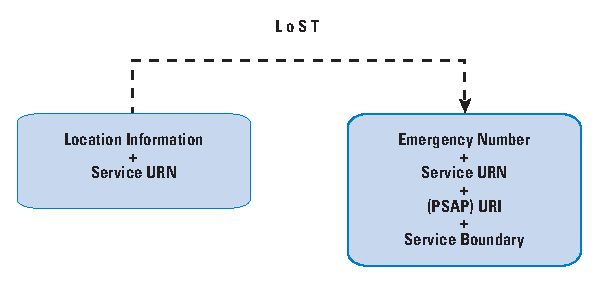
\includegraphics[scale=0.80]{figures/ietf-lost-figure.eps}
 \caption{High-Level Functionality of Location-to-Service Translation (LoST).}
 \label{ietf-lost-figure}
\end{figure}

\subsection{Obligations}

In this section we discuss the requirements the different entities need to satisfy, based on Figure~\ref{ietf-architecture-figure}. A more detailed description can be found in~\cite{draft-ietf-ecrit-phonebcp}. Note that this narration focuses on the final stage of deployment and does not discuss the transition architecture, in which some implementation responsibilities can be re-arranged, with an impact on the overall functionality offered by the emergency services architecture. A few variations were introduced to handle the transition from the current system to a fully developed ECRIT architecture.

\begin{figure}[!t]
 \centering
 \includegraphics[scale=0.60]{figures/ietf-architecture-figure.eps}
 \caption{Main Components involved in an Emergency Call.}
 \label{ietf-architecture-figure}
\end{figure}

With the work on the IETF emergency architecture we have tried to balance the responsibilities among the participants, as described below. 

\subsubsection{End Hosts\\}

An end host, through its VoIP application, has three main responsibilities: it has to attempt to obtain its own location, determine the URI of the appropriate PSAP for that location, and recognize when the user places an emergency call by examining the dial string\index{Dial String}.  The end host operating system may assist in determining the device location.

The protocol interaction for location configuration is indicated as interface (a) in Figure~\ref{ietf-architecture-figure} and a number of location configuration protocols have been developed to provide this capability.

A VoIP application needs to support the Location-to-Service Translation (LoST) protocol~\cite{rfc5222} in order to determine the emergency service dial strings\index{Dial String} and the PSAP URI. Additionally, the \index{service URN}service URNs, defined in~\cite{rfc5031}, need to be understood by the device.

As currently defined, it is assumed that PSAPs can be reached by \index{SIP}SIP, but may support other signaling protocols, either directly or through a protocol translation gateway.  The LoST retrieval results indicate whether other signaling protocols are supported. To provide support for multi-media different types of codecs may need to be supported; details can be found in~\cite{draft-ietf-ecrit-phonebcp}.

\subsubsection{ISP\\}

The ISP has to make location information available to the end point via one or more of the location configuration protocols.

In order to route an emergency call correctly to a PSAP, an ISP may initially disclose the approximate location for routing to the end point and more precise location information later, when emergency personnel is dispatched by the PSAP operator.  The functionality required by the IETF emergency services architecture is restricted to the disclosure of a relatively small amount of location information, as discussed in~\cite{rfc6444} and in~\cite{draft-ietf-ecrit-rough-loc}.

The ISP may also operate a caching LoST server to improve the robustness and the reliability of the architecture. This lowers the roundtrip time for contacting a LoST server, and the caches are most likely to hold the mappings of the area where the emergency caller is currently located.  

In the case where ISPs allow Internet traffic to traverse their network, the signaling and media protocols used for emergency calls function without problems. Today, there are no legal requirements to offer prioritization of emergency calls over IP-based networks. While the standardization community has developed a range of Quality of Service signaling protocols, their widespread deployment still remains to happen.

\subsubsection{VSP\\}

\index{SIP}SIP does not mandate that call setup requests traverse \index{SIP}SIP proxies, i.e., \index{SIP}SIP messages can be sent directly to the user agent. Thus, even for emergency services, it is possible to use \index{SIP}SIP without the involvement of a VSP.  However, in terms of deployment, it is highly likely that a VSP will be used. If a caller uses a VSP, this VSP often forces all calls, emergency or not, to traverse an outbound proxy or session border controller (\index{SBC}SBC) operated by the VSP.  If some end devices are unable to perform a LoST lookup, VSP can provide the necessary functions as a back-up solution. 

If the VSP uses a signaling or media protocol that is not supported by the PSAP, it needs to translate the signaling or media flows.

VSPs can assist the PSAP by providing identity assurance for emergency calls, e.g., using SIP Identity\index{SIP Identity} (RFC 3325~\cite{rfc3325}), thus helping to prosecute prank callers. However, the link between the subscriber information and the real-world person making the call is weak. In many cases, VSPs have, at best, only the credit card data for their customers and some of these customers may use gift cards or other anonymous means of payment. 

\subsubsection{PSAP\\}

The emergency services best current practice document~\cite{draft-ietf-ecrit-phonebcp} only discusses the standardization of the interfaces from the VSP and ISP towards PSAPs and some parts of the PSAP-to-PSAP call transfer mechanisms that are necessary for emergency calls to be processed by the PSAP. Many aspects related to the internal communication within a PSAP, between PSAPs as well as between a PSAP and first responders are beyond the scope of the IETF specification.

When emergency calling has been fully converted to Internet protocols, PSAPs must accept calls from any VSP, as shown in interface (d) of Figure~\ref{ietf-lost-figure}.  Since calls may come from all sources, PSAPs must develop mechanisms to reduce the number of malicious calls, particularly calls containing intentionally false location information. Assuring the reliability of location information remains challenging, particularly as more and more devices are equipped Global Navigation Satellite Systems (GNSS\index{Positioning!GNSS}) receivers, such as GPS, allowing them to determine their own location~\cite{draft-ietf-ecrit-trustworthy-location}. However, it may be possible in some cases to verify the location information provided by an end-point by comparing it against network-provided location information.

\subsection{LoST Mapping Architecture}
\index{LoST Mapping Architecture}
So far, we have described the LoST protocol as it is described in RFC 5222~\cite{rfc5222}, namely as a client-server protocol. A single LoST server, however, does not store the mapping elements for all PSAPs worldwide, for both technical and administrative reasons. Thus, there is a need to let LoST servers interact with other LoST servers, each covering a specific geographical region.  The LoST protocol already provides the baseline mechanisms for supporting such a communication architecture, as described in RFC 5582~\cite{rfc5582}, an informational RFC providing terminology (in the form of different roles for LoST servers that distinguish their behavior) and explaining the basic concept of the LoST mapping architecture. RFC 5582 motivates the basic design decision for LoST to utilize it in a wide variety of architectures, but leaves the detailed instantiation to deployments in different jurisdictions. 

The awareness of peering LoST servers  determines the structure of the architecture rather than certain physical properties of a network, such as topology of a fiber installation, or the structure of a national emergency services organization. Two types of structures are used in combination, namely a mesh and a hierarchical structure. The mesh topology is envisioned for the top-level LoST entities, whereas the hierarchical structure reflects a parent - child relationship in a tree. Figure~\ref{lost-structure-figure} shows this structure graphically with the LoST servers acting in their roles of forest guides (FGs) and trees. A tree consists of a self-contained hierarchy of authoritative mapping servers (AMS) for a particular service. An AMS is a LoST server that can provide the authoritative answer to a particular set of queries. The top-most server in a tree is a tree root and this server peers with one or multiple FGs, i.e., the tree root announces its coverage region to FGs. In Figure~\ref{lost-structure-figure}, for example, the root of tree 1 interacts with FG A and makes the coverage area available. FG A also receives the coverage area from the root of tree 2. All tree roots receive information about the coverage area of their children in the tree. On the top level, all FGs (namely FG A, FG B, and FG C) form a mesh and synchronize their coverage areas. 

\begin{figure}[!t]
 \centering
 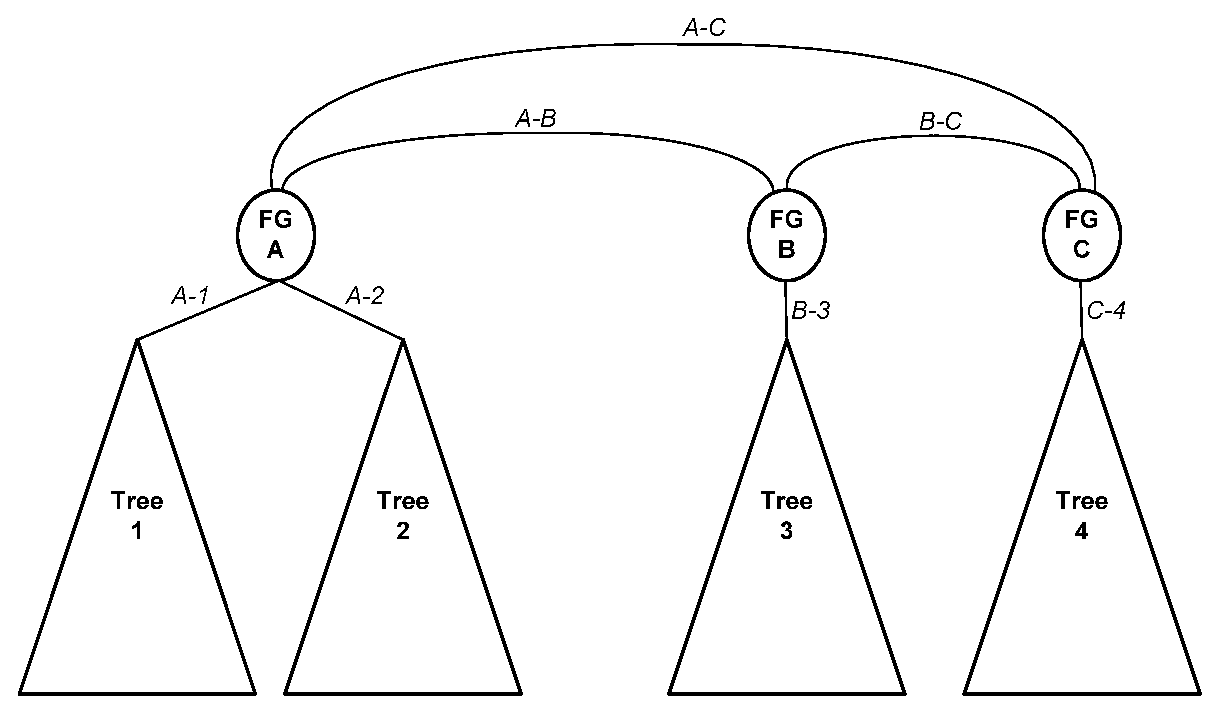
\includegraphics[scale=0.60]{figures/lost-structure-figure.eps}
 \caption{Trees and Forest Guides in the LoST Mapping Architecture.}
 \label{lost-structure-figure}
\end{figure}

Seekers and resolvers are two additional LoST entities in the LoST mapping architecture that are not shown in Figure~\ref{lost-structure-figure}. Neither seekers nor resolvers provide authoritative answers themselves but they may cache results. Particularly the use of resolvers to cache mapping elements is expected to be very common.

To best understand the LoST mapping architecture it is important to highlight the main design goals:

\begin{description}

\item [Robustness: ] To ensure the stability of the system even if different people in different places of the LoST architecture make different decisions, the system will still function. It cannot be assumed that everyone has to agree with everyone else. The minimum level of agreement that has to be ensured is that AMSs are able to authoritatively answer mapping queries, i.e., only those LoST servers respond authoritatively if they indeed have the authority of a specific coverage area. 

\item [Consistent Responses: ]  Any device (called seeker) can issue a LoST query and it will get a consistent answer regardless of where the query enters the system. In some (rare) cases of territorial disputes, two AMSs may claim  authoritative for the same region. In such a case, the answer received by a seeker will vary depending on the entry point into the mapping system. 

\item [Scalability: ] Scalability of the LoST architecture is ensured by the use of caching and the distributed nature of the LoST servers in the architecture. Any LoST entity may support caching of received mapping elements. The mapping elements may be obtained as part of the ordinary operation of LoST (via query and responses) but also via separate replication of the mapping elements. LoST Sync~\cite{rfc6739} is one such protocol to exchange mappings between LoST servers (and other entities).\index{LoST Sync}

\item [Minimal Seeker Configuration:] A seeker is a LoST client requesting a mapping. The only information a seeker needs to know is the address of a resolver; it does not need to know the structure of all Forest Guides nor does it need to maintain a global picture of LoST servers. To avoid having end user involvement in the configuration of LoST servers, Section 4 of the LoST specification provides a discovery technique based on DNS, and RFC 5223~\cite{rfc5223} offers a DHCP-based discovery procedure. Although LoST servers can be located anywhere,  a placement topologically closer to the end host, e.g., in the access network, may be desirable in disaster situations with intermittent network connectivity. RFC 5223 offers this capability.

\end{description}

Even though it is technically possible to let seekers and resolvers enter their queries at any point in the LoST mapping architecture, a deployment choice is to configure resolvers with the addresses of the FGs. A query and response for an emergency caller located in Germany with a service provider in Finland could then be shown as depicted in Figure~\ref{lost-example-query-figure}. In our example we assume that the VSP deploys a LoST resolver that is contacted by the their own customers, the seekers. We furthermore assume in this example that no caching takes place to illustrate the message flow (as shown with dotted lines). In message (1) the seeker contacts its pre-configured resolver with a recursive query providing its current location (somewhere in Germany). The resolver at this point in time does not have any information about the PSAP that has to be contacted for the given location in Germany (for the solicited service). Since the resolver knows the address of the forest guide (only one forest guide is shown in our example), it issues an iterative query to it, as marked with message (2). The FG responds with the entry point for the German LoST tree. The resolver then issues another query towards the provided tree root in message (3). For this example we assume that the root of tree 1 knows the address of the PSAP the seeker has to contact. This final response is then forwarded to seeker via the resolver. The resolver would want to cache the intermediate and final results in order to speed-up later lookups for the same geographical area and the same service. Once the seeker knows the final answer, it can proceed with the emergency call setup procedure to contact the PSAP, as shown in message (4) with the double line. 

\begin{figure}[!t]
 \centering
 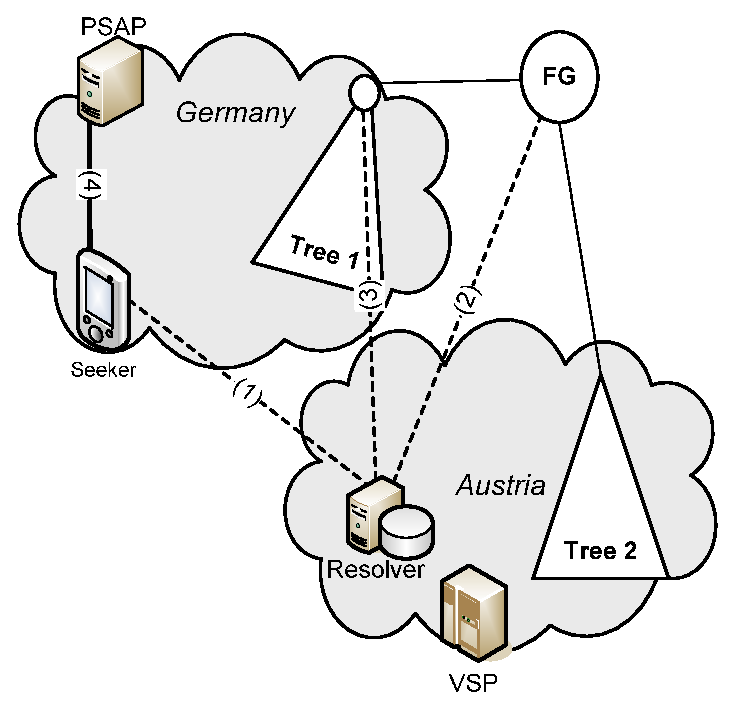
\includegraphics[scale=0.70]{figures/lost-example-query-figure.eps}
 \caption{Example Query / Response in the LoST Mapping Architecture.}
 \label{lost-example-query-figure}
\end{figure}

As illustrated, LoST servers form a distributed mapping database, with each server carrying mapping elements. These mapping elements are the main data structure that is communicated in the LoST protocol, synchronized between FGs and LoST servers in the tree, and cached by resolvers and seekers. Figure~\ref{ietf-mapping-element-figure} shows the data elements of this important data structure graphically.

\begin{figure}[!t]
 \centering
 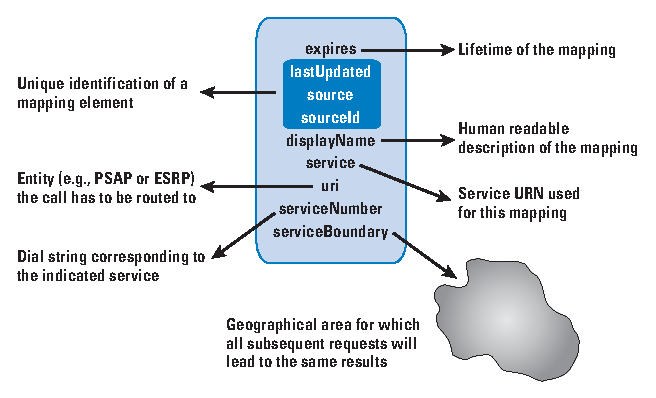
\includegraphics[scale=0.80]{figures/ietf-mapping-element-figure.eps}
 \caption{Mapping Element.}
 \label{ietf-mapping-element-figure}
\end{figure}

\subsection{Steps towards an IETF Emergency Services Architecture}

The architecture described so far requires changes both in already-deployed VoIP end systems and in the existing PSAPs. The speed of transition and the path taken varies between different countries depending on funding and business incentives. As such, it is difficult to argue whether upgrading end points will be easier or replacing the emergency service infrastructure. In any case, the transition approaches being investigated consider both directions. We can distinguish roughly four stages of transition; the description below omits many of the details due to space constraints:
\begin{itemize}
\item Initially, VoIP end systems cannot place emergency calls at all. This is currently the case for many software clients, such as GoogleTalk.
\item In a second stage, VoIP callers manually configure their location, and emergency calls are routed to the appropriate PSAP as circuit-switched calls via \index{PSTN}PSTN gateways, using technologies similar to mobile calls. This level of service is now offered in some countries for \index{PSTN}PSTN-replacement VoIP services, i.e., VoIP services that are offered as replacement for the home phone. In the United States, this is known as the "\index{Organizations and Groups!NENA}\index{NENA!i2}\index{Organizations and Groups!NENA}NENA \index{NENA!i2}i2" service.
\item In a third stage, PSAPs maintain two separate infrastructures, one for calls arriving via an IP network, and the legacy infrastructure.
\item In the final stage, all calls, including those from traditional cell phones and analog landline phones, reach the PSAP via IP networks, with the legacy calls converted to the ECRIT requirements by the carriers or the emergency service infrastructure.
\end{itemize}

\subsubsection{Legacy End Points\\}

Figure~\ref{ietf-mapping-element-figure} shows an emergency services architecture with legacy end points. When the emergency caller dials the European-wide emergency number '112' (step 0), the device treats it as any other call without recognizing it as an emergency call, i.e., the dial string\index{Dial String} provided by the end point that may conform to RFC 4967~\cite{rfc4967} or RFC 3966~\cite{rfc3966} is signaled to the VSP (step 1). Recognition of the dial string is then left to the VSP for processing/sorting; the same is true for location retrieval (step 2) and routing to the nearest (or appropriate) PSAP (step 3). Dial string recognition, location determination and call routing are simpler on a fixed device and voice / application service provided only by the ISP than when they are provided via separate a VSP and ISP. 

If devices are used in environments without location services, the VSP's \index{SIP}SIP proxy may need to insert location information based on estimates or subscriber data. We briefly describe these cases below.

\begin{figure}[!t]
 \centering
 \includegraphics[scale=0.60]{figures/ietf-legacy-endpoints-figure.eps}
 \caption{Emergency Services Architecture with Legacy End Points.}
 \label{ietf-legacy-endpoints-figure}
\end{figure}

There are two main challenges to overcome when dealing with legacy devices: First, the VSP has to discover the \index{LIS}LIS that knows the location of the IP-based end host. The VSP is only likely to know the IP address of that device, which is visible in the call signaling that arrives at the VSP. When a \index{LIS}LIS is discovered and contacted, and some amount of location information is available, then the second challenge arises, namely how to route the emergency call to the appropriate PSAP. To accomplish the latter task, it is necessary to have some information about the PSAP boundaries. 

\cite{draft-ietf-ecrit-phonebcp} does not describe a complete solution for interworking with legacy PSAPs but instead offers building blocks to use. The following constraints exist when dealing with legacy end points: 
\begin{itemize}
\item Only the emergency numbers\index{Emergency Numbers} configured at the VSP are understood. This may lead to cases where a dialed emergency number is not recognized or a non-emergency call is routed to a PSAP. 
\item Using the host's IP address to discover the ISP network to which the host is attached is challenging and may, in case of mobility protocols and \index{VPN}\index{VPN}VPNs, lead to wrong results.
\item Security and privacy concerns may arise when a large number of VSPs/ASPs can retrieve location information from an ISP. It is likely that only authorized VSP/ASPs will be granted access. Hence, it is unlikely that such a solution would work smoothly across national boundaries.
\item When the emergency call is not recognized by the User Agent, then functions like call waiting, call transfer, three way call, flash hold, outbound call blocking, etc. cannot be disabled. 
\item The User Agent software may block callbacks from the PSAP since it does not have ways to recognize those as calls related to an earlier emergency. 
\item Privacy settings may not be respected and identity information may get disclosed to unauthorized parties. These identity privacy features exist in some jurisdiction even in emergency situations.
\item Certain VoIP call features may not be supported, such as a REFER (for conference call and transfer to secondary PSAP) or the Globally Routable User Agent URIs (GRUU) for identifying individual devices issuing the emergency call. 
\item User Agents will not be able to convey location information to the VSP (even if it is available). 
\end{itemize}

\subsubsection{Partially Upgraded End Hosts\\}

A giant step forward in simplifying the handling of IP-based emergency calls is to provide the end host with some information about the ISP so that \index{LIS}LIS discovery is possible. The end host may, for example, learn the ISP's domain name, by using \index{LIS}LIS discovery~\cite{rfc5986}, or might even obtain a Location by Reference (\index{LbyR}\index{LbyR}LbyR) via the DHCP-URI option~\cite{draft-ietf-geopriv-dhcp-lbyr-uri-option} or via \index{HELD}\index{HELD}HELD~\cite{rfc5985}. The VSP is then either able to resolve the \index{LbyR}\index{LbyR}LbyR in order to route the call or to use the domain to discover a \index{LIS}LIS using DNS.

Additional software upgrades at the end device may allow emergency calls to be recognized based on some pre-configured emergency numbers\index{Emergency Numbers} (e.g., '1-1-2' and '9-1-1') and allow for the implementation of other emergency service-related features, such as disabling silence suppression during emergency calls. 

\subsection{Outlook}

Regulation for IP-based emergency services is still at an early stage in most countries. The ability to obtain location information of IP devices automatically is not a requirements in most networks. Automatically obtaining location information is crucial for reliable emergency service operation to support nomadic\footnote{Nomadic devices remain in one place during a communication session, but are moved frequently from place top place. Laptops with \index{WiFi}WiFi interfaces are currently the most common nomadic device.} and mobile devices.

Regulators have traditionally focused on the national or, at most, the European level, and the international nature of the Internet poses new challenges. For example, mobile devices are now routinely used beyond their country of purchase and, unlike traditional cellular phones, need to support emergency calling functionality. It appears likely that different countries will deploy IP-based emergency services over different time horizons, so that a traveler may be surprised to find that she cannot call for emergency assistance outside their home country.

The separation between Internet access and application providers on the Internet is one of the most important differences to existing circuit switched telephony networks. A side effect of this separation is the increased speed of innovation at the application layer, and the number of new communication mechanisms is steadily increasing. Many emergency service organizations have recognized this trend and advocate for the use of new communication mechanisms, including video, real-time text, and instant messaging, to offer improved emergency calling support for citizens. Again, this requires regulators to re-think the distribution of responsibilities, funding and liability.

For many communication systems in use today it is difficult to trace malicious activities back to the human who caused them since identity proofing requirements are often fairly low when registering with Internet application services. This is not a completely new problem, as pay phones and prepaid cell phones have long offered mischief makers the opportunity to place hoax calls, but the weak user registration procedures, the lack of deployed end-to-end identity mechanisms, and the ease of providing false location information increases the attack surface at PSAPs. Attackers also have become more sophisticated over time, and using botnets to generate a large volume of automated emergency calls to exhaust PSAP resources, including call takers and first responders, is not science fiction. 

%\bibliographystyle{wiley}
\bibliographystyle{plain}
\bibliography{references}
%\bibliography{rfc,i-d,internet,references}

%\begin{glossary} 
%  \term{RSVP} TBD.
% \end{glossary}

%\anxx{Fu\, Tschofenig}


%\clearpage
%\addcontentsline{toc}{chapter}{Index}
%\latexprintindex


\end{document}

